\section*{Calibración}

Una curva de calibración se obtiene a travez de un proceso experimental con la finalidad de representar el comportamiento físico del dispositivo en este caso una termocupla mediante el establecimiento de varios punto de temperatura, definiendo 6 valores de temperatura partiendo de la temperatura ambiente a $T_i = 20 C°$ hasta un valor final $T_o = 40C°$.

Los puntos para el rango expresado se muestra en la tabla \ref{tab:vout-circuito-termopar}

\begin{table}[]
	\centering
	\begin{tabular}{|cc|}
		\hline
		\multicolumn{2}{|l|}{\textbf{Calibración Termopar}}               \\ \hline
		\multicolumn{1}{|l|}{\textbf{T{[}c°{]}}} & \textbf{Vout {[}mV{]}} \\ \hline
		\multicolumn{1}{|c|}{20}                 & 38.71                  \\ \hline
		\multicolumn{1}{|c|}{24}                 & 60.25                  \\ \hline
		\multicolumn{1}{|c|}{28}                 & 91.13                  \\ \hline
		\multicolumn{1}{|c|}{32}                 & 126.932                \\ \hline
		\multicolumn{1}{|c|}{36}                 & 162.42                 \\ \hline
		\multicolumn{1}{|c|}{40}                 & 190.158571             \\ \hline
	\end{tabular}
	\caption{Voltaje de salida respecto a la temperatura}
	\label{tab:vout-circuito-termopar}
\end{table}

Y los cuales se usarán para interpolar la curva de calibración al aplicar una regresión lineal la cual se escoge a partir de la tendencia de datos con pendiente positiva la cual se muestra en la figura \ref{fig:graph-vout-temperatura}

Destacando de este procedimiento la obtención de una ecuación de calibración lineal la cual se asemeja al modelo inicial de un termopar el cual se encuentra caracterizado por la variación de la temperatura en relación inversa al coeficiente de seebeck como se muestra en la ecuación \ref{eq:calibracion} 

\begin{equation}
	V_o = 7.854T - 124.02
	\label{eq:calibracion}
\end{equation}

La cual define una razón de cambio de 7.854, encontrando así una sensibilidad de 7.5 $mV$ por unidad de temperatura o su equivalente a $\frac{7.5mV}{C°}$.

\subsection*{Gráfica Vo respecto a la temperatura}

% TODO: \usepackage{graphicx} required
\begin{figure}[h]
	\centering
	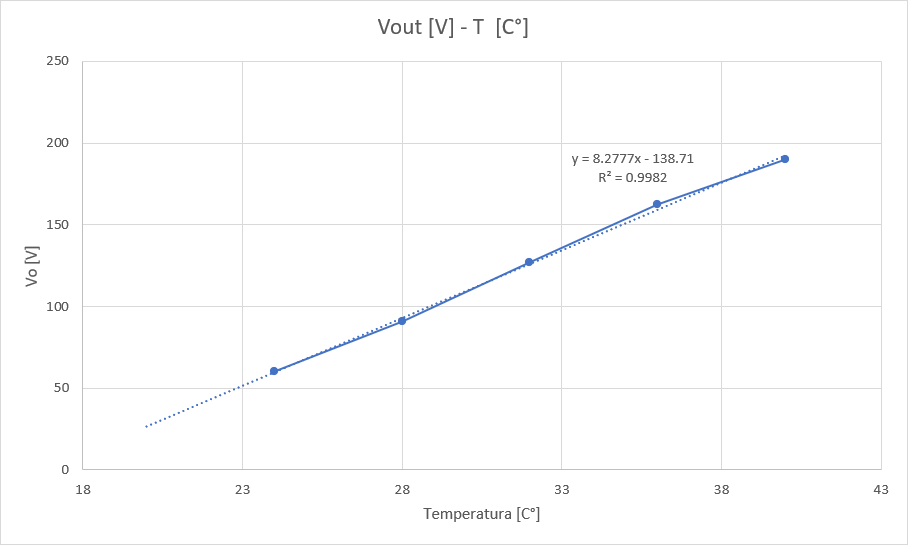
\includegraphics[width=0.8\linewidth]{media/graph-vout-temperatura}
	\caption{Gráfica de relación de temperatura respecto al voltaje}
	\label{fig:graph-vout-temperatura}
\end{figure}